\chapter{Industrial Context and Research Framework}
\minitoc

In this first chapter, we present the context of the Industry 4.0 in which this thesis project is inscribed. Primarily, we will review the industry 4.0 paradigm as well as the benefits it can bring to the manufacturing industry through the application of AI-based data-driven methods. Subsequently we will describe our research framework focused on improving the quality of the parts produced through the Extrusion Blow-Molding process. 

\section{Industry 4.0: a promise for improved manufacturing}

Automotive industry is nowadays driven by global competition and the need for fast adaptation of production to the ever-changing market requests. The fourth revolution in industry, Industry 4.0, holds the promise of increased flexibility in manufacturing, along with mass customization, better quality, and improved productivity \citep{zhong2017intelligent}. 

As already occurred for the past three revolutions, technical innovations and a new way of perceiving the world, are radically changing the industry. The first industrial revolution at the end of the 18th century introduced steam-powered machines. The second one used electricity to improve productivity and to create mass production. Electronics and information technology, with the introduction of Programmable Logic Controllers (PLC) began the industrial automation and the third industrial revolution. The context of billions of people connected by mobile devices, with unprecedented processing power, storage capacity, and access to knowledge is promoting the emergence of new technologies. Artificial intelligence, robotics, autonomous vehicles, 3-D printing, nanotechnology, biotechnology, materials science, energy storage, and quantum computing are changing the world and today we are on the cusp of the fourth industrial revolution \citep{schwab20164th}.  

The term Industry 4.0 refers to the connection among production departments, tools, machines, “individual things” in general made possible by Internet and CPS (cyber physical systems) \citep{schlapfer2015industry} .
With the digital revolution, the boundaries between the physical and digital worlds are disappearing to create an interconnected factory with strong interactions between employees, machines and products. These connected entities can interact with one another using standard Internet-based protocols and analyze data to predict failure, configure themselves, and adapt to changes.
According to the estimations made by BCG for German companies, Industry 4.0 will have a positive impact on companies with productivity and revenue growth but also on economy with more investments and with an overall six percent increase in employment during the next ten years. Productivity improvements on conversion costs, which exclude the cost of materials, will range from 10 to 20\% in automotive industry, while productivity gains of 5 to 8\% will be achieved if the materials costs are factored in. 
The revenue growth, as a direct consequence of  Manufacturers demand for enhanced equipment and new data applications, as well as consumer demand for a wider variety of increasingly customized products, is estimated at 30€ billion a year, which is approximately one percent of the German GDP \citep{russmann2015industry}. 

Industry 4.0 is also a new way of looking at performance, with a more precise and immediate vision (based on real-time indicators) of the entire production chain, but also the optimization of production through the use of artificial intelligence. In the context of an interconnected plant, the large amount of data collected from different sources—production equipment and systems as well as enterprise—can be helpful in taking decision and contributes to a continuous improvement process. In particular, we think that the integration of machine learning models inside our complex industrial processes can reduce the non-quality costs with the increase of the overall equipment effectiveness (OEE). 
% Explain how the AI is one of the most import technology --> do the link with the next section


\subsection{Data}

In the last decades, computers and any kind of Information Technology (IT) Resources occupy a central place in almost every manufacturing industry. The "Big Data" paradigm is a consequences of the improvement of three IT technologies: Data storage, Network and Computing power. The continuous reduction in price of Data storage capacity and Computing power technologies are encouraging the manufacturing industry to rethink their IT architecture putting the data at the heart 

% Architettura importante cosi come un approccio sistematico per il recupero dei dati

\subsubsection{The importance a centralized data storage}

In contrast with the previous points suggesting a vast amount of data available for analysis, industrial data applications may face data accessibility issues that might also limit the feasibility any data analysis process. The data may come from different sources

\subsubsection{The Manufacturing data}

% Structured vs Unstructured

Industrial data comes in very different forms and forms. This implies a lot of heterogeneity in the data which tend to complexity any data usage or comparison. Moreover, most of the data available in the manufacturing industry is \textit{Unstructured}. 

\begin{definition}[label=structured]{Structured Data}
In this thesis we consider as structured any kind of data that can be stored in form of rows and columns in systems like databases or Excel Spreadsheet. Any data that can be stored by respecting this convention, without loosing any information, can be qualified as a structured data.
\end{definition}

\begin{definition}[label=unstructured]{Unstructured Data}
 On the other hands, we consider as Unstructured any set of data that cannot be stored in a set of rows and columns without losing inner information. 
\end{definition}

Some types of data may be difficult to definitely classify into one or the other category. It could actually depend on the use-case and the data processing objective. For example, an image can be represented as a 2D matrix (for black and white images) or as 3D matrix (for colour images). This representation is a perfectly structured. Therefore an image, or a video, could be considered as a structured data format for someone willing to conduct a spectral analysis, only interested in the pixel values and positions. Nonetheless, the same image can also be considered unstructured if we focus our interest on the content of the image. Indeed, pixel values can not be easily translated into a structured representation of the actual content.
Nonetheless, someone willing to extract design intents from these files will probably argue a different point of view considering the difficulty to access this implicit information. Moreover relying on hypothetical metadata, with varying quality and content, can not be considered as a viable systematic solution to this problem, therefore justifying that many engineering standardized formats could, in fact, be considered as unstructured data formats, under specific objectives, despite being implemented in perfectly structured and standardized data formats.

Unfortunately, dealing with unstructured data is a lot more challenging in a data science perspective \citep{blumberg2003problem}\citep{sagiroglu2013big} \citep{buneman1997adding}. It requires highly complex, expensive and time-consuming feature extraction processes and operations (i.e. a feature represents a descriptor (e.g. colour of a car) in a data science context). It is estimated that the average \textit{Information Systems} (IS) roughly contain around 15\% of structured data and 85\% of unstructured data. Such an assumption seems consistent with the actual status of the manufacturing industry. Furthermore, even if a more optimistic situation is considered, with a balanced rate of 50\% structured and 50\% unstructured data, it still appears critical to be able to mine, explore, exploit, and search in these data. Consequently, we could state that a Big Data context is inherently linked to unstructured data.
Dealing with engineering data implies to use and manage large amounts of human-made data. These data come with inherent and recurring issues which highly limit their usability without an extensive pre-processing.


\subsection{Machine Learning and Artificial Intelligence}

As highlighted before in the previous section, the amount of available data is exponentially increasing and thus it can be reasonably considered that humans will not be able any more, in a near future, to process, by hand, these massive amounts of data and perform heavy computations in a parallel manner. Nonetheless, software products based on AI algorithms, take advantage of parallel computation capabilities and large data quantities to approach human behaviors and understanding in complex situations.

The presence of an increasing volume of data opens up new research and improvement perspectives. How we take advantage of this data ?  

Industrial AI is not just a reuse of general AI technology in the industrial domain. Within industry, the characteristics of fragmentation, individualization and specialization
of problems determine that Industrial Intelligence depends on the deep integration of computer science, AI, and domain knowledge. Unlike traditional methods of rule-based or mechanism-based modeling, one of the major advantages of data-driven Industrial Intelligence technology is the ability to establish predictive analysis based on insight and evidence contained in the data, which allows for establishing smart management tools for invisible problems and exploring the relationships between complex things. This way, new knowledge is accumulated to form an intelligent system which can be continuously iterated on.

\subsubsection{History}
In last decade, the hottest machine learning sub-field, Deep Learning has gained a lot of popularity due to the ability to provide state-of-the-art results in multiple domains: from web searches, to image recognition and detection through Convolutional Neural Networks, to natural language processing with Recurrent Neural Networks and, more recently Self-Attention based Neural Networks. Deep Learning is not a new idea, most of the recent proposed Deep Learning architectures are built using discoveries from the last years of the 20th century. Since the founding of AI as a field of research at the 1956 Dartmouth Workshop until the year 2000, AI experienced two “AI winters.” The first began in 1973, represented by the publishing of the Lighthill Report. Because of the gap between anticipated AI progress and real results, the US government cut funds to AI research. In the following decade, AI was hardly mentioned; but in the 1980s, because of the emergence of FINISH
AI has received new attention again in 2012 when Alex Krizhevsky and his colleagues used deep learning technology \citep{krizhevsky2012imagenet} on ImageNet for the first time to outperform other teams, making people aware of the advantages of deep learning over traditional machine learning, bringing deep learning to the forefront for the first time. 

The reborn popularity of these computational methods can be attributed to the following reasons:

\begin{itemize}
    \item \emph{Increasing Computer Power}: Deep learning networks are known to be computationally intensive FINIRE. 
    Moreover, the availability of Cloud Computing solutions at an affordable price
    \item \emph{Larger labeled datasets}: The explosion of Big Data in the last decade, has considerably increased the size of the dataset available inside the manufacturing companies. The availability of an important amount of data is indispensable for the successful application of Deep learning methods because these methods require, in average, more data compared to conventional Machine learning approaches. 
    \item \emph{Advances in Deep Learning research}: Deep Learning is one of the research domain FINIRE . As pointed by the "AI index 2019 report" \citep{zhang2021ai}, between 1998 and 2018, the volume of peer-reviewed AI papers has grown by more than 300\%, accounting for 3\% of peer-reviewed journal (Figure \ref{fig:Number of Peer-Reviewed AI Publications}) publications and 9\% of published conference papers.
    \item \emph{Open source tools and models}: 
\end{itemize}

\begin{figure}
\centerline{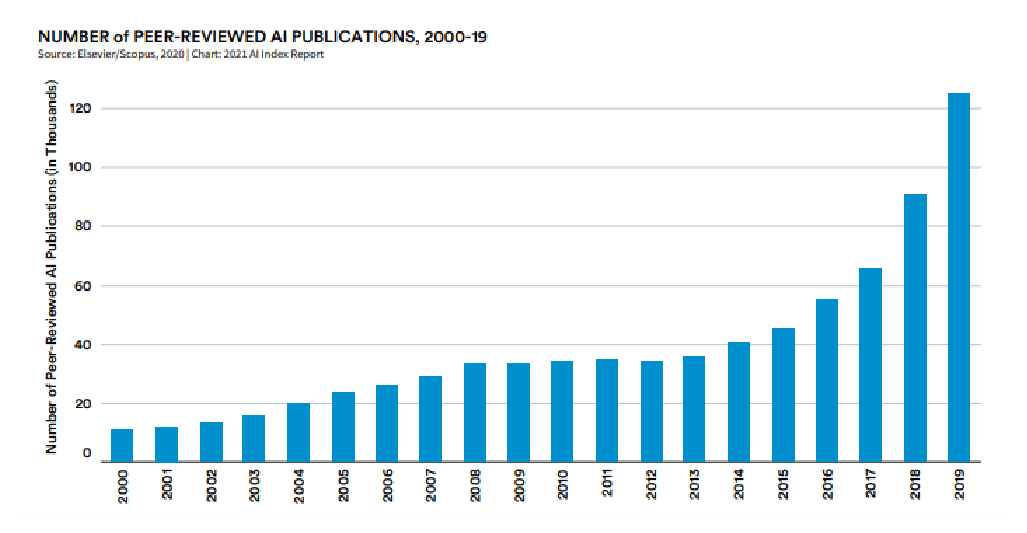
\includegraphics[scale=0.9]{images/chapter_1/AI_report.eps}}
\caption{Number of Peer-Reviewed AI Publications, 2000-2019 \citep{zhang2021ai}}
\label{fig:Number of Peer-Reviewed AI Publications}
\end{figure}

% Change
At the same time, graphics processing unit (GPU) replaced central processing unit (CPU) in computer vision training, shortening the length of training from several months to a few days or hours. Breakthroughs in hardware, algorithms, and big data in various fields brought an explosion in AI growth.



\subsubsection{Review of opportunities for the manufacturing industry}

In this section we presents the result of a research review we conducted to highlight some of the possibles applications where the Machine Learning could be applied in order to create value for the manufacturing companies. This study should not, in any case, be considered as an exhaustive list of possibilities. Results are summarized in table \ref{tab:ai_benefits}. 

\begin{table}
\caption{AI benefits in Manufacturing}
\label{tab:ai_benefits}
\begin{tabular}{|l|p{6cm}|p{4cm}|}
\hline
%
Domain &
  Benefits &
    Bibliography \\ \hline
% Quality Optimization
Quality Optimization &
  Decrease the product failure rate at the end of the production line. Optimize key performance index of the final product to meet customer needs. &
    \citep{lieber2013quality}\citep{li2018ensemble}\citep{chen2008neural}\citep{nagorny2017quality}\citep{haeussler1996quality} \\ \hline
Product failure detection &
  Detects the products that do not meet the standard of production. The failure product is not counted in the final production volume. A high failure rate leads to low production volume. &
    
    \\ \hline
Maintenance &
  Increase the availability of the production line by preventing the breakdown of equipment in advance. Predict the risk of malfunction of the production line and arrange proactive maintenance. &
    \citep{nguyen2019new}\citep{lee2017application}\citep{einabadi2019dynamic}\citep{li2017intelligent}\citep{liu2016prediction}\\ \hline
Fault Diagnosis &
  Prognostic diagnose of production line failure event. Identify the malfunction part of the production line. Predict the abnormal behaviors of machines and equipment. \\ \hline
Scheduling Optimisation &
  Logistic management of the production line, which can maximize the throughput of the production line. Buffer control and product routing management. \\ \hline
\end{tabular}
\end{table}

\subsubsection{Challenges of AI in Industry}

Although AI technology has made breakthroughs in many applications, there is still a big gap between large-scale usage in industrial scenarios. This is because industry and manufacturing value stability, standardization, accuracy, and repeatability, as well as mechanization, processes, operations, and close integration of process requirements \citep{lee2020industrial}. Before AI technologies can be fully integrated into industrial systems, it is necessary to overcome the challenges of reproducibility, reliability, and security

\paragraph{Reproductibility}

% TO REVIEW

Unfortunately, this practice is not widely adopted by researchers in the manufacturing research
communities. Too few datasets are actually available to conduct research. It can be assumed that
the lack of opened datasets is probably induced by the secretive policies frequently enforced in the manufacturing industry. Unfortunately, this tends to hinder research possibilities and produce the following unwanted side-effects:

\begin{itemize}
    \item Very difficult, if not impossible, to reproduce any claimed result in the state-of-the-art. This highly limits the effectiveness of peer-reviewing.
    \item Very difficult, if not impossible, to compare the proposed approaches to address a specific problem. Aside of qualitative studies, there is no common metric based on a shared dataset to evaluate and rank the different methods.
    \item Developing a dataset may literally cost millions of dollars. If every researcher or research group needs to build a new one from scratch, the developing costs will be are multiplied.
    \item Small research laboratories may not be able to work on some research topics due to a lack of funds available to build a decent dataset. This situation may namely affect the emerging countries.
\end{itemize}



\paragraph{Data issues}


Concerning data, AI technology out the manufacturing industry faces five major challenges and limitations: 

\begin{enumerate}
    \item Training data is heavily dependent on manual work, otherwise it is difficult to obtain a large and comprehensive training data set, and the quality of labeling is heavily dependent on human experience and ability.
    \item The transparency of the model needs
    to be improved since AI algorithms cannot explain how conclusions are reached step-by-step.
    \item Models are not very general, and it is hard to replicate from one application to the next. This means lots of money and energy is needed to train new models for new problems.
    \item The risk of deviation in data and algorithms, much
    like the differences between societies and culture, requires extensive steps to solve.
    \item It is difficult to reach agreement on data privacy and attribution.
\end{enumerate}

\paragraph{Reliability}

% TO REVIEW

According to the different requirements of reliability in different domains and applications, AI can be roughly divided into mission-critical and non-mission-critical applications. Currently, most AI products on the market do not require strict system reliability. As long as a certain threshold of usability is reached, the occasional errors and problems can be tolerated without serious consequences in non-mission-critical applications. For critical applications, if a system has even a small chance of failure, it could lead to serious consequences, causing property loss or even harm to human beings or social stability. This is particularly true for all those applications that have to do with the safety of people. An example of this is the intelligent driving industry: it is expected
that this industry will globally reach \$9.5 billion by 2020. The industry is facing serious challenges in guaranteeing safety. The first fatal drone crash occurred in March of 2018, and an Uber autopilot test car hit and killed a woman in May of 2018. Whether it is true autonomous driving technology or a driving assistance system, its high demand for reliability and intolerance of failures makes it difficult for the technology to truly enter the market before exceeding the human driving level. These challenges are the same in industrial systems. If we want to employ AI technology to control the functioning of an entire system, we must be extremely cautious about mission-critical tasks, which necessitates not just advancements in model and algorithm accuracy, but also security limits and uncertainty management in system design. For instance, for a manufacturing company with low percentage of quality scraps, an AI model with a 80\% accuracy in prediction may lead to incorrect alerts FINIRE 


\section{The research framework: The Extrusion Blow Molding}


The industrial process taken into account for our experimental setting is the Extrusion Blow-Moulding process. Extrusion blow molding is a process used to form hollow thermoplastic objects (especially bottles and containers). The process takes a thin-walled tube called a \textit{parison} that has been formed by extrusion, entraps it between two halves of a larger diameter mold, and then expands it by blowing air into the tube, forcing the parison out against the mold. The outside of the thin-walled part takes the shape of the inside of the mold \citep{poli2001design}.

\begin{figure}
\centerline{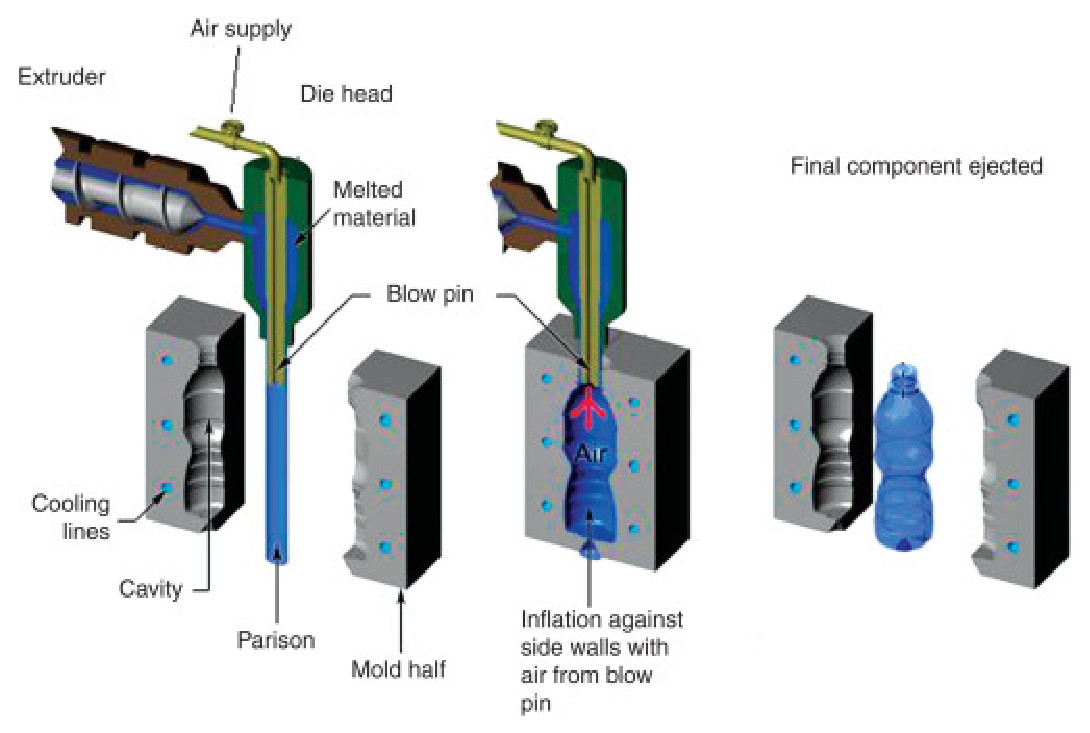
\includegraphics[scale=0.75]{images/chapter_1/extrusion_blow_molding.eps}}
\caption{Extrusion Blow-Molding \citep{goodship2015design}}
\label{fig:Extrusion Blow-Molding}
\end{figure}

As easily guessed by the name, the Extrusion Blow-Molding process is composed of two sub-processes: Extrusion and Blow-Molding.

\begin{itemize}
    \item \textit{The Extrusion:} The Extrusion is a continuous-flow process where a plastic material feedstock is fed through a hopper onto a feeding transfer screw. The thermal energy provided by the heating clamps as well as the mechanical energy provided by the screw rotation allow the melting of the plastic material. The molten material is then pressure fed through a arranged in a vertical position such that the resulting extruded molten parison is hanging vertically from the die. The die will typically create a tubular extruded cross-section, round or oval depending upon the final shape of the finished blow molded part.
    \item \textit{The Blow-Molding:} Unlike Extrusion, Blow-Molding is a discontinuous-flow process where FINIRE. Once the blow operation is completed and the part has frozen suitably for ejection, the mold opens and the part is ejected, allowing the extruded parison to be extruded through the mold for the next cycle. 
\end{itemize}

Each phase has parameters that influence the subsequent phases and, ultimately, the characteristics of the finished product. The multiple phases mean that the number of parameters that can be adjusted on the process is fairly high. It is possible to fine-tune temperatures, screw speeds and throughputs for the Exttrusion, as well as the  pressure curves, molds opening and closing times for the Blow-Molding phase. In addition, the Extrusion Blow-moulding process has a certain dynamic: it takes a certain amount of time for the adjustment of one of the process parameters to have an effect on the products. This dynamic is mainly due to the thermal inertia of the solid tooling.
One of the most critical part of the process is the parison formation. In fact, the dimensions of the blow molded article are directly related to the dimensions of the parison. Furthermore, the thermo-mechanical history of the material during the parison formation stage and the resulting weight and diameter distribution of the parison have a great influence on the characteristics of the subsequent inflation and cooling stages. The shape and the dimensions of the parison are the result of complex interactions between the molten ploymer and the thermo-mechanical conditions that influence the melt after it leaves the extruder die. Parison formation it is affected by two phenomena knows as \textit{swell} and \textit{sag}. Parison swell, occurring both in diameter and thickness, is due to the nonlinear viscoelastic deformation of the polymer melt in the extrusion die. Sag is caused by gravitational forces that act on the suspended parison \citep{huang2002prediction}. A high degree of swell could lead to molded articles which are to heavy and uneconomical, on the other hands, very low swelling could yield incomplete parts of low weight with unacceptable wall thickness.

There are many variations of this process including equipment made to extrude multiple parisons simultaneously, equipment that can extrude multiple layers within the same parison, equipment with rotary capability that will hold several molds and can provide a continuous nonstop process, equipment which shuttles tools into and away from the parison, and the list goes on. In the context of this thesis project we have mainly worked with a Blow-Molding process, whose finished products are obtained from the overlay of multiple plastic layers. This particular type of Blow-Molding process takes the name of \textit{Co-extrusion}. Co-extrusion was born out of the need of reduce the permeability of fuel tanks. For plastic fuel tanks it is mandatory to comply with a set of security norms, .
The steps for producing a multi-layers plastic product are the same as those used by the traditional single layer process, except for the number of extruders involved in the manufacturing process. Up to six extruders can be used simultaneously to melt different plastic materials. The goal is to create a multi-layer tank with the use of different material, as shown in
Figure \ref{fig:Co-extrusion Process}

\begin{figure}
\centerline{\includegraphics[scale=0.55]{images/chapter_1/coextrusion.png}}
\caption{Co-extrusion Process}
\label{fig:Co-extrusion Process}
\end{figure}

Extrusion Blow Molding is a less expensive process than injection blow moulding and can provide a wide variety of barriers and features such as handles, but the dimensional accuracy is not as well controlled. By controlling variations in the parison thickness along its length, the wall thickness of the final part can be approximately controlled. From an industrial point of view, the Extrusion Blow-Molding process is a high-speed, low-cost, repeatable process. Once the FINIRE

The Extrusion Blow-Molding constitutes one of the various stages necessary to produce the finished part. The stages needed to manufacture a finished part may vary depending on the type of product made. For instance, a fuel tank container, a plastic bottle or a plastic bumper may requires different post-production processes. Further information on how the fuel tank are FINIRE are available in Appendix \ref{Full production process}. As far as our thesis work is concerned, we will only focus on The Extrusion Blow Molding stage.

% Talk about continuous extrusion

\subsection{The key parameters of the Extrusion Blow-Molding}

The following table resume the list of the key parameters of an extrusion blow-molding process.

% Put table in landscape view
\begin{landscape}
\begin{table}[]
\caption{Blow-Molding Key parameters}
\label{tab:key_parameters}
\begin{tabular}{|l|l|l|l|l|l|}
\hline
Process      & Parameter            & Unity of measure & Value range   & Description                 & Dependencies \\ \hline
Extrusion    & Speed*               & RPM              & {[}0, 90{]}   & Rotation speed of the screw &              \\ \hline
Extrusion    & Throughput*          & Kg/h             &               &                             &              \\ \hline
Extrusion    & Feeding Temperature* & °C               &               &                             &              \\ \hline
Extrusion    & Melt Temperature*    & °C               &               &                             &              \\ \hline
Extrusion    & Cycle time           & s                & {[}60, 120{]} &                             &              \\ \hline
Extrusion    & Parison profile      &                  &               &                             &              \\ \hline
Blow-Molding & Blowing pressure**   &                  &               &                             &              \\ \hline
Blow-Molding &                      &                  &               &                             &              \\ \hline
Blow-Molding &                      &                  &               &                             &              \\ \hline
\end{tabular}
\end{table}
\end{landscape}

\subsection{The Quality of an extruded blow-molded part}

Quality Control is generally expressed as a management activity verifying the conformity of the process and the product/service to the requirements that constitute its quality standard. The ISO 9000 standard defines quality control as "A part of quality management focused on fulfilling quality requirements". In the industrial context taken into account the requirements are defined by the customers. Several characteristics are measured on the product and compared with the customer requirements, if the measures are compliant with the customer specifications the part can be sent to the customer, otherwise the part have to be rejected. 
In the framework of the Extrusion Blow-Molding process, we are mostly interested in the dimensional/geometric characteristics. In fact, 


The following table resume some of the specific tests that have to be carried to the blow-molded parts to ensure their conformity to the customer specifications.

% Insert Blow-Molding table

\section{Industrial problem: Improving Quality}

Because manufacturing processes are becoming more and more complex, and the high level of requirement in the automotive industry regarding safety and environmental impacts, Plastic Omnium is continuously seeking for innovation throughout its different projects: that allows the company to remain leader in its field.
For an equipment manufacturer like Plastic Omnium Clean Energy Systems, bad or ``scrap'' parts are very expensive for the company. The “Cost of Non-Quality” (CNQ) is one of the key indicators most used by the company. However, when a part is bad, it is first necessary to understand the origin of the problem, which can require a lot of time and energy.



\section{Contributions: Towards new quality control framework}

Manufacturing Industries non quality costs are mainly due to product scraps, when they are not compliant with the customer specifications and to Quality Recalls, due to to the sale of parts found to be non-conforming when used by the customer. Hopefully Quality Recall are not  % Dovuta ai pezzi scartati e ai Recall clienti

Our dissertation develops along two major axes: the process improvement and the quality control improvement. We claims that the improving of the overall quality of a production line can be obtained by working either on the process and either on the quality control. 

Improving the process FINIRE

Improving the quality control means 

This thesis has, in our opinion three main contributions:

\begin{itemize}
    \item It provides a general framework to improve the Process Control of complex Manufacturing process. We propose a data-driven approach which take advantage of the historical data to try to model the relationship between process parameters and the quality of a product. Our approach, presented in Chapter 3 is compose of 4 main stages: the data acquisition, the data processing, the Machine Learning modeling and the FINIRE. The four stages 
    \item It provides a general framework to improve the Quality Control. Using a data-driven approach we can use sensors, cameras or any kind of equipment to collect meaningful data. This approach open ups new possibilities in term of Quality Control.  
    \item In Chapter 4, we propose an approach to infer the thickness of Blow-Molded parts using thermal imaging and a Deep Learning without any direct measurement of the part.   
\end{itemize}


\section{Conclusion}

In this first chapter we have highlighted the context in wh

\subsection{Scientific Contribution}

\subsection{Industrial Contribution}

In this chapter we have seen that we are on the cusp of the 4th industrial resolution. Industry 4.0, holds the promise of increased flexibility in manufacturing, along with mass customization, better quality, and improved productivity. The development of new technologies such us the AI, the IoT are opening up new perspective in the Manufacturing Industry. AI in particular seems able to take advantage of the fast growing amount of data available in the manufacturing plants to FINIRE 
